\chapter{Introduction to Systems Programming in Linux Computing Environment}
\section{Introduction}
\subsection{Objectives}
This lab is to introduce system programming in a general Linux Development Environment at ECE Department. After finishing this lab, students will be able to
\begin{itemize}
   \item apply basic Linux commands to interact with the Linux system through shell;
   \item apply standard Linux C programming tools for system programming and
   \item create a program to interact with Linux file systems by applying the relevant system and libray calls.
\end{itemize}

\subsection{Topics}
Concretely, the lab will cover the following topics:
\begin{itemize}
  %\item how to connect to a remote Linux server;
  \item Basic Linux commands
  \item C programming toolchain including \verb+gcc+, \verb+make+, and \verb+ddd+
  \item Linux manual pages
  \item Linux system calls and file I/O library calls to traverse a directory and perform read/write operations on selected files.
  \end{itemize}
  
\section{Starter Files}

The starter files are on GitHub at url: \url{http://github.com/yqh/ece252/tree/master/lab1/starter}.
It contains the following sub-directories where we have example code and image files to help you get started:
\begin{itemize}
    \item the \href{http://github.com/yqh/ece252/tree/master/lab1/starter/cmd_arg}{cmd\_arg} demonstrates how to capture command line input arguments;
    \item the \href{http://github.com/yqh/ece252/tree/master/lab1/starter/images}{images} contains some image files;
    \item the \href{http://github.com/yqh/ece252/tree/master/lab1/starter/ls}{ls} demonstrates how to list all files under a directory and obtain file types;
    \item the \href{http://github.com/yqh/ece252/tree/master/lab1/starter/png_util}{png\_util} provides a set of utility functions to process a PNG image file;
    \item the \href{http://github.com/yqh/ece252/tree/master/lab1/starter/pointer}{pointer} demonstrates how to use pointers to access a C structure; and
    \item the \href{http://github.com/yqh/ece252/tree/master/lab1/starter/segfault}{segfault} contains a broken program that has a segmentation fault bug, which you will debug in the last Pre-lab exercise.
\end{itemize}
Using the code in the starter files is permitted and will not be considered as plagiarism.

\section{Pre-lab Preparation}

%Read Chapter \ref{ch_linux_env}. 
Read the Introduction to ECE Linux Programming Environment supplementary material in Part \ref{part_ref} Chapter \ref{ch_linux_env}. Do the pre-lab exercises in Section \ref{sec_ex1}. Finish the pre-lab programming assignment before your scheduled lab starts (see \ref{sec:lab1_prelab_assignment}).
\subsection{Basic Linux Commands Exercises}
\label{sec_ex1}

These pre-lab exercises are to practice some basic commands on Linux. 
\begin{enumerate}
    \item Use the MobaXterm to login onto
      \code{eceubuntu.uwaterloo.ca}. You are now inside the Linux shell and in your home directory. The home directory usually has a path name in the format of \verb+/home/username+, where username normally is your UWID. For example, a user with UWID of \verb+jsmith+ has a home directory of \verb+/home/jsmith+.
    \item Use the \code{pwd} command to print the full filename of the current working directory. You should see your home directory name printed on the screen. For example: \verb+/home/jsmith+.
    \item Use the \code{echo \$HOME} command to print your home directory path name. You will notice that the output matches the \verb+pwd+ output of exercise 2.
    \item Use the \code{env} command to list all the environment variables and their values. Note that \verb+HOME+ is one of the many environment variables.
    \item One important environment variable is \verb+PATH+. It specifies a set of directories the system searches for executible programs. Use \code{echo \$PATH} to see your \verb+PATH+ environment variable setting.
    \item Execute command \code{which ls} to locate the directory the ls command is in. You will notice the directory is listed in \verb+PATH+ environment variable. When you issue a command and get an error message of ``command not found'', it means the command cannot be found after searching all the directories listed in \verb+PATH+ environment variable. A commonly seen error is that a command in your current working directory gives you ``command not found`` error. This is normally due to the fact that the current working directory \verb+.+ or \verb+./+ is not in the PATH. Consequently you need to add the path to the command name for the system to know where the command is. For example \code{./a.out} tells the system to run the command \verb+a.out+ located in the current working directory. 
    \item Use the \code{ls} command to list all files in your current working
          directory. 
    \item Read the online manual of the \verb+ls+ command by issuing 
      \code{man ls} command to the shell.
      Find out from the manual what options \verb+-l+, \verb+-a+ and \verb+-la+ do.
      Execute  the \verb+ls+ command with these three options and see the execution results.
    \item Create a directory as the work space of labs under your home directory. 
          Name the newly created directory as \verb+labs+.
          Read the man page of the command \verb+mkdir+ to see how to do it.
    \item Change directory to the newly create directory of \verb+labs+.
          Read the man page of command \verb+cd+ to find out how to change directory.
    \item Clone the ece252 lab repository by using the command: \\
      \code{git clone https://github.com/yqh/ece252.git}.

      A new directory named \verb+ece252+ will be created. It has lab manual and starter code of ECE252 labs. 
    \item Read the man page of the \verb+find+ command by issuing   
      \code{man find} command to the shell. Read what the \verb+-name+ option does. Use \verb+find+ with the \verb+-name+ option to find all the files with .png file extension in the \verb+$HOME/labs/ece252+ directory.
    \item Change directory to where the \verb+WEEF_1.png+ is. Use \code{file WEEF\_1.png} command to obtain the file type and image properties such as dimensions and bit depth.
    \item Use \verb+file+ command to obtain the file type information of \verb+Disguise.png+. You should see that this is not an image file though the file exension is .png.  Use a text editor to open the file and see the contents. This exercise is to show you that the \verb+file+ command does not obtain the file type information based on the file extension. It looks into the contents of file to extract the file type information
      %REV%\footnote{A file has a magic number to indicate its type. The magic number is a sequence of bytes usually appearing near the beginning of the file. The file command checks the magic number. The PNG file's magic number is 89 50 4E 47 OD 0A 1A 0A in hexadecimal format. It is interesting to notice that the second, third and fourth characters are P N and G in ASCII.}.
      \footnote{A file has a magic number to indicate its type. The magic number is a sequence of bytes usually appearing near the beginning of the file. The file command checks the magic number. The PNG file's magic number is 89 50 4E 47 in hexadecimal, which is .PNG in ASCII.}.
    \item You can use the command \verb+display+ to display an image. For example, to view the \verb+WEEF_1.png+ file, use the command \verb+display WEEF_1.png+. 
    \item Execute \code{cat red-green-16x16.png} command and you will notice the output are gibberish funny characters. This is because cat displays plain text file in a human readable form, not a binary file. The PNG image file is a binary file. Both vi and emacs have hexadecimal mode which displays the bytes in binary files in a hexadecimal format. They are pretty good for small size binary files. There are also few linux commands that perform hex dump of a file. The \verb+xxd+ is one of them. Try \code{xxd red-green-16x16.png} and see the output. Other similar commands include \verb+od+ and \verb+hexdump+. Refer to the man pages of these commands for detailed usage instructions. 
    \item The \verb+pngcheck+ command test PNG image files for corruption. Some image viewers are able to display the image even part of the data are corrupted. An image can be opened by an image viewer does not guarantee it is not corrupted. You will notice that the \verb+display+ command will not display a corrupted PNG image file on Linux. But the same corrupted image file most likely can be displayed by Windows Paint program. Execute the following two commands and see what pngcheck output tells you.
      \begin{itemize}
      \item \code{pngcheck red-green-16x16.png}
      \item \code{pngcheck red-green-16x16-corrupted.png}
      \end{itemize}
    \item Images are binary files. To compare two binary files, we can use the \verb+cmp+ command. Read the man page of the \verb+cmp+ command and especially pay attention to the \verb+-l+ option. Use the \verb+cmp+ command with the \verb+-l+ option to find out which bytes in \verb+red-green-16x16.png+ and \verb+red-green-16x16-corrupted.png+ are different. Another tool is \verb+vbindiff+, which displays and compares hexadecimal file(s).  
     \item Use gdb or ddd to run the program under \url{http://github.com/yqh/ece252/tree/master/lab1/starter/segfault} directory of the starter code. When the code generates a segmentation fault inside the debugger, run the gdb command \code{where} to see the stack trace and fix the segmentation fault problem of the code. 
\end{enumerate}

\subsection{Pre-lab Assignment}
\label{sec:lab1_prelab_assignment}
We will write some small pieces of code that can be used in the final lab assignment code. We will create a command line program named \verb+pnginfo+ that prints the dimensions of a valid PNG image file and an error message to the standard output if the input file is not a PNG file or is a corrupted PNG file. The command takes one input argument, which is the path name of a file. Both absolute path name and relative path name are accepted. For example, command \code{./pnginfo WEEF\_1.png} will output the following line: 
\begin{verbatim}
WEEF_1.png: 450 x 229 
\end{verbatim}
If the input file is not a PNG file. Then output an error message. For example, command \code{./pnginfo Disguise.png} will output the following line:
\begin{verbatim}
Disguise.png: Not a PNG file 
\end{verbatim}
If the input file is a PNG file, but certain chunks has CRC error. That is the CRC value in the chunk does not match the CRC value computed by your program, then the program output something similar as what pngcheck does. For example, command \code{./pnginfo red-green-16x16-corrupted.png} will output the following line:
\begin{verbatim}
red-green-16x16-corrupted.png: 16 x 16 
IDAT chunk CRC error: computed 34324f1e, expected dc5f7b84
\end{verbatim}

You will find starter files under \href{http://github.com/yqh/ece252/tree/master/lab1/starter/png_util}{png\_util} directory are helpful. To make our pre-lab code reusable in the final lab, we will create two functions. One is \verb+is_png()+ which takes eight bytes and check whether they match the PNG image file signature. Another function is \verb+get_data_IHDR()+ which extracts the image meta information including height and width from a PNG file IHDR chunk. You are free to design the signatures of these two functions so that they will be re-used in your lab1 final solution and future labs 2 and 3 solutions\footnote{lab2 and lab3 are based on the code of lab1}. However in \verb+lab_png.h+ you will find some existing function prototypes that we put there to show one possible function prototype design. Feel free to modify these function prototypes to fit your own design. For computing the CRC of a sequence of bytes, the starter file already provides the crc.c and crc.h and the main.c that demos how to call the crc function to do the computation.
\section{Lab Assignment}
\subsection{Problem statement}

\begin{wrapfigure}{r}{2.5in}
  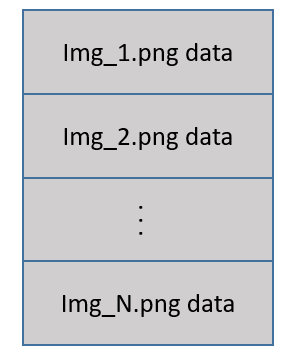
\includegraphics[width=2in]{img/img_concatenation}
  \caption{Image Concatenation Illustration}
\label{fig_img_concatenation}
\end{wrapfigure}

You are given a directory under which some files are PNG images and some files are not. The directory may contain nested sub-directories\footnote{A nested sub-directory is a sub-directory that may contain many layers of sub-directories.}. All valid PNG images under the given directory are horizontal strips of a bigger whole image. They all have the same width. The height of each image might be different. The PNG images have the naming convention of \verb+*_N.png+, where \verb+N+ is the image strip sequence number and \verb+N=0, 1, 2, ...+. However a file with .png or .PNG extension may not be a real PNG image file. You need to located all the real PNG image files under the given directory first. Then you will concatenate these horizontal strip images sequentially based on the sequence number in the file name to restore the original whole image. The sequence number indicates the order the image should be concatenated from top to bottom. For example, file \verb+img_1.png+ is the first horizontal strip and \verb+img_2.png+ is the second horizontal strip. To concatenate these two strips, the pixel data in \verb+img_1.png+ should be followed immediately by the pixel data in \verb+img_2.png+ file. Figure \ref{fig_img_concatenation} illustrates the concatenation order.

To solve the problem, first you will create a tool named \verb+findpng+ to search the given directory hierarchy to find all the real PNG files under it. Secondly you will create an image data concatenation tool named \verb+catpng+ to concatenate pixel data of a set of PNG files to form a single PNG image file. The \verb+catpng+ only processes PNG images with the same width in dimension.
\subsection{The findpng command}
The expected behaviour of the \verb+findpng+ is given in the following manual page of the command.
\subsubsection{Man page of findpng}
\subsubsection*{NAME}
\begin{itemize}
	\item[]{\bf findpng} - search for PNG files in a directory hierarchy
\end{itemize}
\subsubsection*{SYNOPSIS}
\begin{itemize}
	\item[]{\bf findpng} DIRECTORY 
\end{itemize}
\subsubsection*{DESCRIPTION}
\begin{itemize}
	\item[]Search for PNG files under the directory tree rooted at DIRECTORY and return the search results to the standard output. The command does not follow symbolic links.
\end{itemize}
\subsubsection*{OUTPUT FORMAT}
\begin{itemize}
	\item[]The output of search results is a list of PNG file relative path names\footnote{It is relative to the command input directory path name}, one file pathname per line. The order of listing the search results is not specified. If the search result is empty, then output ``findpng: No PNG file found''.
\end{itemize}
\subsubsection*{EXAMPLES}
\begin{itemize}
	\item[]{\bf findpng .}
	\item[]Find PNG of the current working directory. A non-empty search results might look like the following:
	\begin{verbatim}
	lab1/sandbox/new_bak.png
	lab1/sandbox/t1.png
	png_img/rgba_scanline.png
	png_img/v1.png
	\end{verbatim}
    It might also look like the following:
	\begin{verbatim}
	./lab1/sandbox/new_bak.png
	./lab1/sandbox/t1.png
	./png_img/rgba_scanline.png
	./png_img/v1.png
	\end{verbatim}
	An empty search result will look like the following:
	\begin{verbatim}
	findpng: No PNG file found
	\end{verbatim}
\end{itemize}
\subsubsection{Searching PNG files under a given directory}
UNIX file system is organized as a tree. A file has a type. Three file types that this assignment will deal with are regular, directory and symbolic link.  A PNG file is a regular file. A directory is a directory file. A link created by \verb+ls -n+ is a symblic link. Read the section 2 of \code{stat} family system calls man page for information about other file types. The \verb+ls/ls_ftype.c+ in the starter code gives a sample program to determine the file type of a given file. Note that the \verb+struct dirent+ returned by the \verb+readdir()+ has a field \verb+d_type+ that also gives the file type information. However it is not supported by all file system types. We will be using eceubuntu machines to test your submission. If you want to use the \verb+d_type+ in your code, make sure you test its behaviour on eceubuntu machines.

To search all the files under a given directory and its subdirectories, one need to traverse the given directory tree to its leaf nodes.  The library call of \code{opendir} returns a directory stream for \code{readdir} to read each entry in a directory. One need to call \code{closedir} to close the directory stream once operations on it is completed. The control flow is to go through each entry in a directory and check the file type. If it is a regular file, then further check whether it is a PNG file by comparing the first 8 bytes with the PNG file header bytes (see Section \ref{subsec_PNG_File_Format}). If it is a directory file, then you need to check files under the sub-directory and repeat what you did in the parent directory.
% The  \verb+chdir()+ family system calls change a working directory.
The \verb+ls/ls_fname.c+ in the starter code gives a sample program that lists all file entries of a given directory.
%The \verb+chdir/chdir1.c+ in the starter code gives one example of how to use the \verb+chdir()+ system call. 

Always check the man page of the systems calls and library calls for detailed information.


\subsection{The catpng command}

The expected behaviour of the \verb+catpng+ is given in the following manual page of the command.
\subsubsection{Man page of the catpng}
\subsubsection*{NAME}
  \begin{itemize}
    \item[]{\bf catpng} - concatenate PNG images vertically to a new PNG named all.png
  \end{itemize}
\subsubsection*{SYNOPSIS}
  \begin{itemize}
    \item[]{\bf catpng} [PNG\_FILE]... 
  \end{itemize}
\subsubsection*{DESCRIPTION}
  \begin{itemize}
  \item[]Concatenate PNG\_FILE(s) vertically to all.png, a new PNG file.
  \end{itemize}
\subsubsection*{OUTPUT FORMAT}
  \begin{itemize}
  \item[]The concatenated image is output to  a new PNG file with the name of all.png.
  \end{itemize}
\subsubsection*{EXAMPLES}
\begin{itemize}
\item[]
\begin{verbatim}
catpng ./img1.png ./png/img2.png
\end{verbatim}
\item[]Concatenate the listed PNG images vertically to all.png.
\end{itemize}

\subsubsection{File I/O}
There are two sets of functions for file I/O operations under Linux. At system call level, we have the {\em unbufferred I/O} functions: \code{open}, \code{read}, \code{write}, \code{lseek} and \code{close}. At library call level, we have standard I/O functions: \code{fopen}, \code{fread}, \code{fwrite}, \code{fseek} and \code{fclose}. The library is built on top of unbufferred I/O functions. It handles details such as buffer allocation and performing I/O in optimal sized chunks to minimize the number of \code{read} and \code{write} usage, hence is recommended to be used for this lab.

The \code{fopen} returns a FILE pointer given a file name and the mode. A PNG image file is a binary file, hence when you call \code{fopen}, use mode "\code{rb}" for reading and "\code{wb+}" for reading and writing, where the "b" indicates it is a binary file that we are opening. Read the man page of \code{fopen} for more mode options. 

After the file is opened, use \code{fread} to read the number of bytes from the stream pointed by the FILE pointer returned by \code{fopen}. Each opened file has an internal state of file position indicator. The file position indicator sets to the beginning of the file when it is just opened. The \code{fread} operation will advance the file position indicator by the number of bytes that has been read from the file. The \code{fseek} sets the file position indicator to the user specified location. The \code{fwrite} writes user specified number of bytes to the stream pointed by the FILE pointer. The file position indicator also advances by the number of bytes that has been written. It is important to call \code{fclose} to close the file stream when I/O operations are finished. Failure to do so may result in incomplete files.  

The man pages of the standard I/O library is the main reference for details including function prototypes and how to use them.   

\subsubsection{PNG File Format}
\label{subsec_PNG_File_Format}
In order to finish this assignment, one need to have some understanding of the png file format and how an image is represented in the file. One way to store an image is to use an array of coloured dots referred to as {\em pixels}. A row of pixels within an image is called a {\em scanline}. Pixels are ordered from left-to-right within each scanline. Scanlines appear top-to-bottom in the pixel array. In this assignment, each pixel is represented as four 8-bit
\footnote{Formally, we say the image has a bit depth of 8 bits per sample.}
unsigned integers (ranging from 0 to 255) that specify the red, green, blue and alpha intensity values. This encoding is often referred to as the RGBA encoding. RGB values specify the colour and the alpha value specifies the opacity of the pixel. The size of each pixel is determined by the number of bits per pixel. The dimensions of an image is described in terms of horizontal and vertical pixels. 

% For each PNG pixel, there are five kinds of information namely read, green ,blue, greyscale, and alpha. A {\em channel} is an array of all per-pixel information of one of these five kinds. For example, the red channel is the array of red values of
\begin{figure}[h]  
\centering
\subfigure[PNG File Format] {
  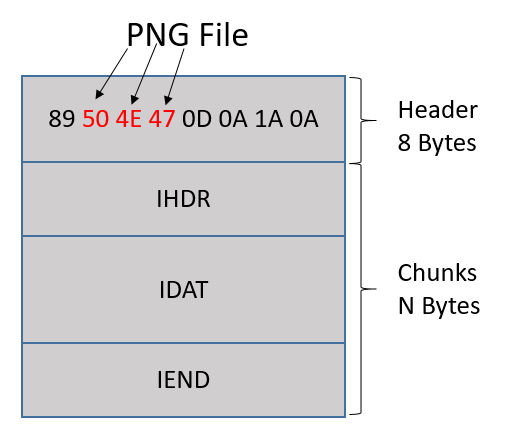
\includegraphics[width = 3in]{img/png_file_format}
  \label{fig_png_file_format}
}
\subfigure[PNG Chunk Format] {
  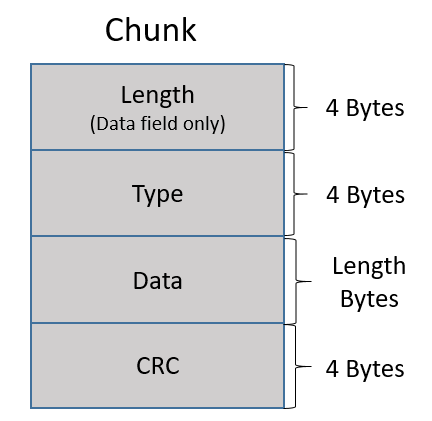
\includegraphics[width = 2.5in]{img/png_chunk_format}
  \label{fig_png_chunk_format}  
}
\end{figure}

PNG stands for ``Portable Network Graphics''. It is a computer file format for storing, transmitting and displaying images\cite{Roelofs1999PNG}. A PNG file is a binary file. It starts with an 8-byte header followed by a series of chunks. You will notice the second, third and fourth bytes are the ASCII code of 'P', 'N' and 'G' respectively (see Figure \ref{fig_png_file_format}).

The first chunk is the IHDR chunk, which contains meta information of the image such as the dimensions of the pixels. The last chunk is always the IEND chunk, which marks the end of the image datastream. In between there is at least one IDAT chunk which contains the compressed filtered pixel array of the image. There are other types chunks that may appear between IHDR chunk and IEND chunk. For all the PNG files we are dealing with in this assignment, we use the format that only has one IHDR chunk, one IDAT chunk and one IEND chunk (see Figure \ref{fig_png_file_format}).


Each chunk consists of four parts. A four byte length field, a four byte chunk type code field, the chunk data field whose length is specified in the chunk length field, and a four byte CRC (Cyclic Redundancy Check) field (see Figure \ref{fig_png_chunk_format}).

The length field stores the length of the data field in bytes. PNG file uses {\em big endian} byte order, which is the network byte order. When we process any PNG data that is more than one byte such as the length field, we need to convert the network byte order to host order before doing arithmetic. The \code{ntohl} and \code{htonl} library calls convert a 32 bit unsigned integer from network order to host order and vice versa respectively.



The chunk type code consists four ASCII character. IHDR, IDAT and IEND are the three chunk type code that this assignment involves with.

The data field contains the data bytes appropriate to the chunk type. This field can be of zero length.

The CRC field calculates on the proceeding bytes in the type and data fields of the chunk. Note that the length field is not included in the CRC calculation. The \code{crc} function under the \verb+png_util+ starter code can be used to calculate the CRC value.
\begin{wraptable}{r}{3in}
	%\begin{table}
	\begin{center}
		\begin{tabular}{llc}             \toprule
			Name               & Length  & Value \\ \midrule
			Width              & 4 bytes & N/A\\ \midrule
			Height             & 4 bytes & N/A\\ \midrule
			Bit depth          & 1 byte  & 8\\ \midrule
			Colour type        & 1 byte  & 6\\ \midrule
			Compression method & 1 byte  & 0\\ \midrule
			Filter method      & 1 byte  & 0\\ \midrule
			Interlace method   & 1 byte  & 0\\ \bottomrule
		\end{tabular}
		\caption{IHDR data field and value}
		\label{lab1:tb_IHDR_Data}
	\end{center}
	%\end{table}
\end{wraptable}
The IHDR chunk data field has a fixed length of 13 bytes and they appear in the order as shown in Table \ref{lab1:tb_IHDR_Data}. Width and height are four-byte unsigned integers giving the image dimensions in pixels. You will need these two values to complete this assignment. Bit depth gives the number of bits per sample. In this assignment, all images have a bit depth of 8. Colour type defines the PNG image type. All png images in this assignment have a colour type of 6, which is truecolor with alpha (i.e. RGBA image). The image pixel array data are filtered to prepare for the next step of compression. The Compression method and Filter method bytes encode the methods used. Both only have 0 values defined in the current standard. The Interlace method indicates the transmission order of the image data. 0 (no interlace) and 1 (Adam7 interlace) are the only two defined. In this assignment, all PNG images are non-interlaced. Table \ref{lab1:tb_IHDR_Data} Value column gives the typical IHDR values the PNG images you will be processing.  

The IDAT chunk data field contains compressed filtered pixel data. For each scanline, first an extra byte is added at the very beginning of the pixel array to indicate the filter method used. Filtering is for preparing the next step of compression. For example, if the raw pixel scanline is 4 bytes long, then the scanline after applying filter will be 5 bytes long. This added one byte per scanline will help to achieve better compression result. After all scanlines have be filtered, then the data are compressed according to the compression method encoded in IHDR chunk. The compressed data stream conforms to the zlib 1.0 format.

The IEND chunk marks the end of the PNG datastream. It has an empty data field.

\subsubsection{Concatenate the pixel data}
To concatenate two horizontal image strips, the natural way of thinking is to start with the pixel array of each image and then concatenate the two pixel arrays vertically. Then we apply the filter to each scanline. Lastly we compress the filtered pixel array to fill the data field of the new IDAT chunk of the concatenated image. However a simpler way exists. We can start with the filtered pixel data of each image and then concatenate the two chunks of filtered pixel data arrays vertically, then apply the compression method to generate the data field of the new IDAT chunk.

How do we get filtered pixel data from a PNG IDAT chunk? Recall that the data field in IDAT chunk is compressed data that conforms to zlib format 1.0. We can use zlib functions to uncompress(i.e. inflate) the data. The \code{mem\_inf} in the starter code takes in memory compressed(i.e. deflated) data as input and returns the uncompressed data to a another memory location. For each IDAT chunk you want to concatenate, call this function and stack the returned data in the order you wish and then you have the concatenated filtered pixel array. To create an IDAT chunk, we need to compress the filtered pixel data. The \code{mem\_def} function in the starter code uses the zlib to compress (i.e. deflate) the input in memory data and returns the deflated data. The \verb+png_util+ directory in the starter code demos how to use the aforementioned two functions.

To create a new PNG for the concatenated images, IHDR chunk also needs to have the new dimension information of the new PNG file. The rest of the fields of IHDR chunk can be kept the same as one of the PNG files to be concatenated. In this assignment, we assume that \verb+catpng+ can only process PNG files whose IHDR chunks only differ in the height field. So the new image will have a different height field, the rest of fields are the same as the input images.



\section{Deliverables}
\subsection{Pre-lab deliverables}
\label{lab1_prelab_deliverable}
Pre-lab is due by the time that your scheduled lab sessions starts. No late submission of pre-lab is accepted. Grace days are not applicable to pre-lab submissions. The following are the steps to create your pre-lab deliverable submission.
\begin{itemize}
\item Create a directory and name it lab1-pre.
\item Put the entire source code with a Makefile under the directory lab1-pre. The Makefile default target includes \verb+pnginfo+. That is command \verb+make+ should generate the aforementioned executable file. We also expect that command \verb+make clean+ will remove the object code and the default target. That is the \verb+.o+ files and the executable file should be removed.
\item Use \verb+zip+ command to zip up the contents of lab1-pre directory and name it lab1-pre.zip. We expect \verb+unzip lab1-pre.zip+ will produce a \verb+lab1-pre+ sub-directory in the current working directory and under the \verb+lab1-pre+ sub-directory is your source code and the Makefile.
\end{itemize}
Submit the \verb+lab1-pre.zip+ file to Lab1 Pre-lab Dropbox in Learn by the time your scheduled lab session starts. The TA on duty will evaluate the pre-lab by letting you demo the submitted program during the scheduled lab session.

\subsection{Post-lab Deliverables}
Post-lab is due two days after your scheduled lab session at 22:00. Grace days can be used towards late submissions of the post-lab deliverable. The following are the steps to create your post-lab deliverable submission.
\begin{itemize}
\item Create a directory and name it lab1.
\item Put the entire source code with a Makefile under the directory lab1. The Makefile default target includes \verb+catpng+ and \verb+findpng+. That is command \verb+make+ should generate the aforementioned two executable files. We also expect that command \verb+make clean+ will remove the object code and the default target. That is the \verb+.o+ files and the two executable files should be removed.
\item Use \verb+zip+ command to zip up the contents of lab1 directory and name it lab1.zip. We expect \verb+unzip lab1.zip+ will produce a \verb+lab1+ sub-directory in the current working directory and under the \verb+lab1+ sub-directory is your source code and the Makefile.
\end{itemize}
Submit the \verb+lab1.zip+ file to Lab1 Dropbox in Learn.
\section{Marking Rubric}
\begin{table}[ht]
\begin{center}
\begin{tabular}{|p{2cm}|p{2cm}|p{9cm}|}
\hline
Points & Sub-points &Description  \\ \hline
15     &   & Pre-lab      \\ \hline
       & 2 & \verb+Makefile+ correctly builds and cleans \\ \hline
       & 13& Implementation of \verb+pnginfo+ \\ \hline
%       & 3 & \verb+ckpng+ detects a non-png file type \\ \hline
%       & 5 & \verb+ckpng+ prints non-corrupted png image dimensions \\ \hline
%       & 5 & \verb+ckpng+ detects incorrect CRC of the simple PNG data chunk \\ \hline
85     &        & Post-lab \\ \hline
       & 10     & Makefile correctly builds and cleans \\ \hline
       & 30     & Implementation of \verb+findpng+  \\ \hline
       & 45     & Implementation of \verb+catpng+ \\ \hline
\end{tabular}
\caption{Lab1 Marking Rubric}
\label{tb_lab1_rubric}
\end{center}
\end{table}

Table \ref{tb_lab1_rubric} shows the rubric for marking the lab. Note that if your code generates a segmentation fault, the maximum lab grade you can achieve is 60/100.

%%% Local Variables:
%%% mode: latex
%%% TeX-master: "main_book"
%%% End:
